\documentclass{article}

\usepackage{arxiv}
\usepackage[ruled,vlined]{algorithm2e}
\usepackage[utf8]{inputenc}
\usepackage[T1]{fontenc}
\usepackage{url}
\usepackage{booktabs}
\usepackage{amsfonts}
\usepackage{nicefrac}
\usepackage{microtype}
\usepackage{graphicx}
\usepackage[font=small,labelfont=bf]{caption}
\usepackage{cite}
\usepackage{pdflscape}
\usepackage{listings}
\usepackage{outlines}

\title{Notes on replication in Apache Kafka}

\begin{document}

\section{Log truncation}

Replication in Kafka evolved from high watermark to log end offset truncation \cite{KIP101} and eventually prevented log divergence under both clean and unclean leader election \cite{KIP279}.

Through log truncation, Kafka ensures replica lineage remains identical and prevents pre-KIP-279 divergences. It relies on the sequence of vectors of \textit{leader epoch} \footnote{also referred to as \textit{generation} in this document} to start offset to ensure replicas are constructed to follow the same lineage.

When a replica starts to follow a leader, the head of its local log is truncated so that remains only the longest common log prefix of the follower and leader replica. In order to do so, the replication algorithm resolves the \textit{fetch offset} the follower must use to start replicating. It searches the latest generation common to both replicas and truncate to the minimum of their respective end offsets. This algorithm is \textit{collaborative} because both leader and follower contributes to the search.

Figure \ref{fig:offsets-for-leader-epoch} exhibits the different steps taken by the algorithm after a sequence of fast broker failovers. In this scenario, two brokers and replicas of a topic-partition are considered and unclean leader election is enabled.

\begin{outline}[enumerate]
	\1 Replica 0 is initially the leader and appends one record to its local log.
	\1 Replica 0 goes offline. Replica 1 is back online and is allowed to acquire leadership because unclean leader election is enabled. One record is appended.
	\1 Broker 1 is bounced. Note that generation is incremented when broker 1 leaves and rejoins the cluster.
	\1 Three back-to-back unclean leader elections happen with leadership alternating between brokers 0 and 1 which remain isolated.
	\1 As broker 1 is the leader, broker 0 becomes online and initiates replication from broker 1.
	\1 Replica 0 first enters the truncation state. The follower sends a \texttt{OffsetsForLeaderEpoch} with the latest generation on the follower, 7. The leader searches for that generation in its local epoch cache. Since it was not online at generation 7, that epoch is not found and the leader returns the largest epoch smaller than 7 it is aware of, or 5, along with its end offset, which is defined as the start offset of the generation directly following generation 5, which is 2 in this case (from the vector $(9,2)$).
	\1 The follower tries to find the epoch 5 in its local epoch cache, but, since it was offline at that generation, uses the largest previous generation contains in its sequence of epochs, or 1. The end offset for that epoch is the start offset of the directly successing epoch, which is 1 from the vector $(7,1)$.
	\1 The follower sends another \texttt{OffsetsForLeaderEpoch} request to inquire about the end offset of the leader for epoch 1. The leader is not aware of that epoch, and in that case, does not contain any epoch smaller than it. It therefore returns the same epoch along with the start offset of the first epoch registered in its local sequence of epochs, or 0 from the vector $(3,0)$.
	\1 The follower observes an epoch from the leader which matches the epoch requested (1), therefore base its fetch offset off of that epoch, using the minimum end offset found for that epoch locally and remotely resolved, or offset 0 in this case.
	\1 The follower deletes all records with offset greater or equal to 0 and starts replicating from that offset.
\end{outline}

Figure \ref{fig:leader-epoch-cache} illustrates the iterative process used to resolve the fetch offset in this example, and shows how the leader and follower collaborates. The offset for epoch 7 is first requested (1), the vector $(5,2)$ is returned by the leader (2), leading the follower to resolve the vector $(1,1)$ (3), then requesting the end offset for that epoch from the leader which responds with vector $(1,0)$ (4), eventually converging to the fetch offset 0 (5).

\begin{figure}[h!]
	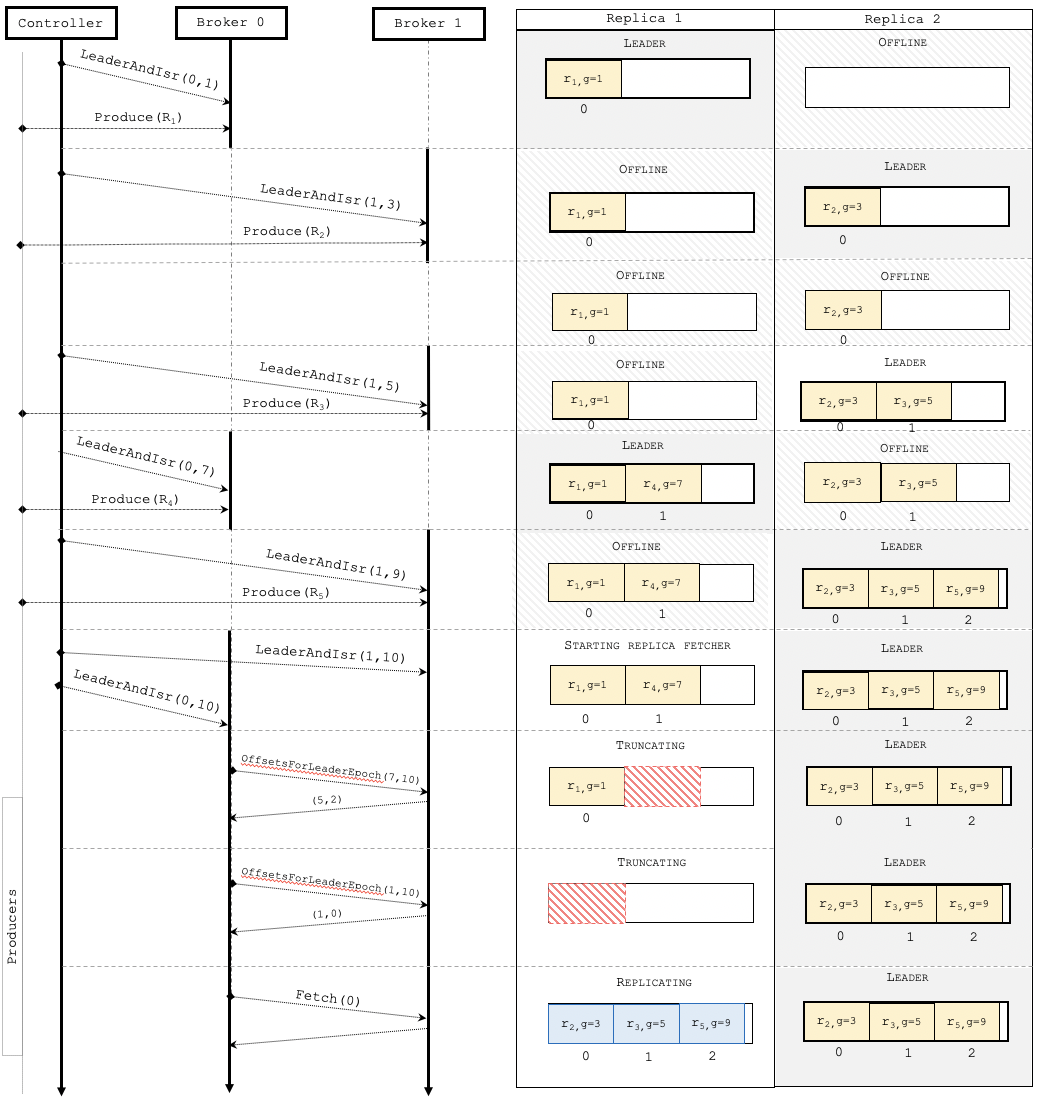
\includegraphics[scale=0.53]{img/offsets-for-leader-epoch.png}
	\captionof{figure}{Back-to-back unclean leader elections resulting in transiently diverging replicas, eventually reconverging through log truncation.}
	\label{fig:offsets-for-leader-epoch}
\end{figure}

\begin{figure}[h!]
	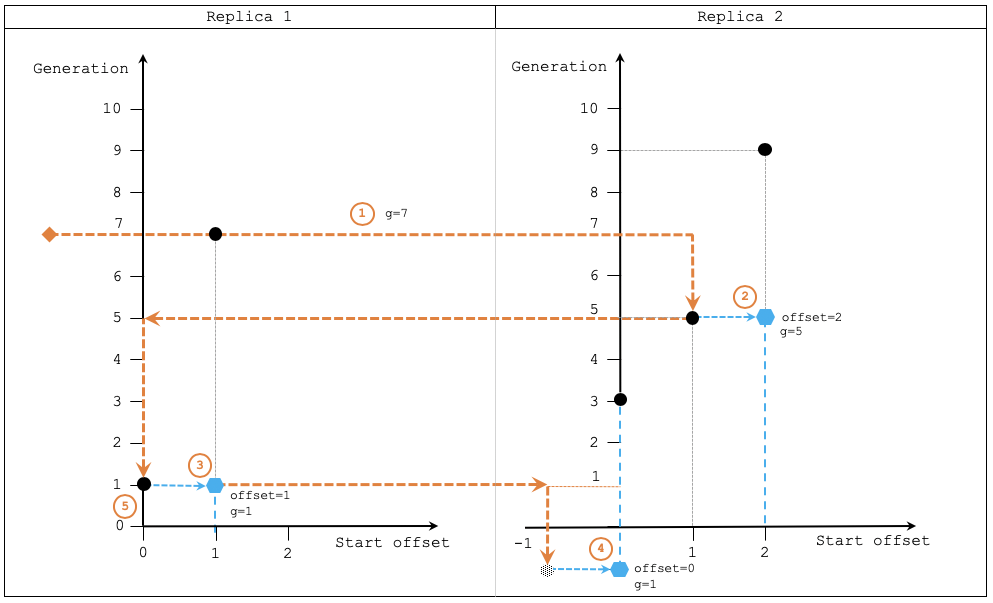
\includegraphics[scale=0.53]{img/leader-epoch-cache.png}
	\captionof{figure}{Collaborative round-trips between a leader and follower to resolve the offset to truncate the follower replica to.}
	\label{fig:leader-epoch-cache}
\end{figure}

\bibliography{kafka-replication}{}
\bibliographystyle{plain}
\end{document}


